\documentclass[../main.tex]{subfiles}

\graphicspath{{\subfix{../imgs/}}}

\begin{document}

\section{Part 1 - Modelling and Simulations}

\subsection{Task 1.1}

Draw a complete equivalent circuit model of the buffer hip including all the signals of the drivers outputs, GDN and VCC supplies, the associated package parasitics for each of the paths and the PCB transmission lines including termination components.

\solution

To fully model the circuit for maximum accuracy we will have to create lumped element models for the supply, driver, receiver and probe. The transmission line will simply be modelled with a time delay and characteristic impedance.

\subsubsection{Supply Model}

The lumped element model for the supply is seen in Figure \ref{fig:supply} and component descriptions (as well as where we find their values) are summarized in Table \ref{tab:supply}.

\begin{figure}[h]
    \centering
    \fbox{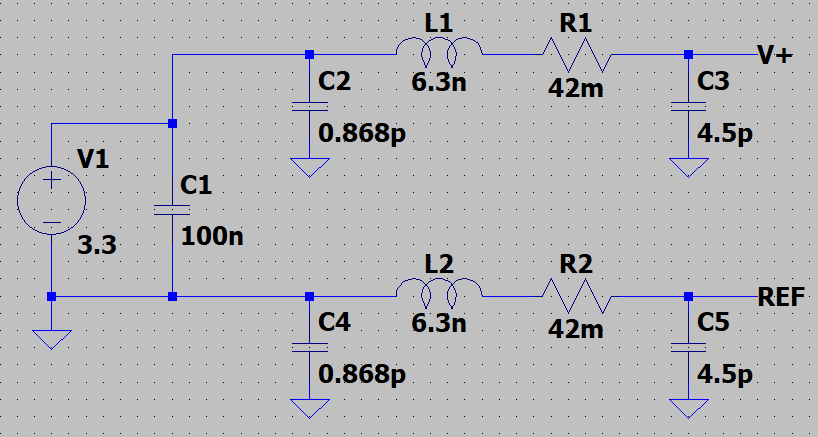
\includegraphics[width=0.8\textwidth]{supply.png}}
    \caption{LTSpice supply model.}
    \label{fig:supply}
\end{figure}

\begin{table}[h]
    \centering
    \begin{tabular}{l|l r}
        \toprule[1pt]
        \textbf{Component} & \textbf{Description} & \textbf{Source}\\
        \midrule
        $C_1$       & Supply decoupling & (Board schematic) \\
        $C_2/C_4$   & 74ALVC244 VCC/GND pin capacitance & (IBIS) \\
        $L_1/L_2$   & 74ALVC244 VCC/GND pin inductance & (IBIS) \\
        $R_1/R_2$   & 74ALVC244 VCC/GND pin resistance & (IBIS) \\
        $C_3/C_5$   & 74ALVC244 input pin capacitance & (Datasheet) \\
        \bottomrule[1pt]
    \end{tabular}
    \caption{Supply model components descriptions.}
    \label{tab:supply}
\end{table}

\subsubsection{Driver/Receiver Model}

Next we model the driver, receiver and transmission line inbetween. Shown in Figure \ref{fig:driver} and summarized in Table \ref{tab:driver}. The buffer likely has a \textit{totem-pole} CMOS pair as the output stage. We model this with switches. The switches have an on resistance of $R_{on} = 1\si{\Omega}$ and an off resistance of $R_{off} = 10^6\si{\Omega}$. The driver has an output capacitance of $C_{driver} = 6.03\si{pF}$ and the receiver has an input capacitance of $C_{receiver} = 4.21\si{pF}$. The time delay of the transmission is determined from the propagation speed listed in assignment 1, $\text{TD} = 0.1 \si{m} / 1.59 * 10^8\si{m/s} = 0.629 \si{ns}$. We assume the transmission line has $Z_0 = 50\si{\Omega}$.

\begin{figure}[h]
    \centering
    \fbox{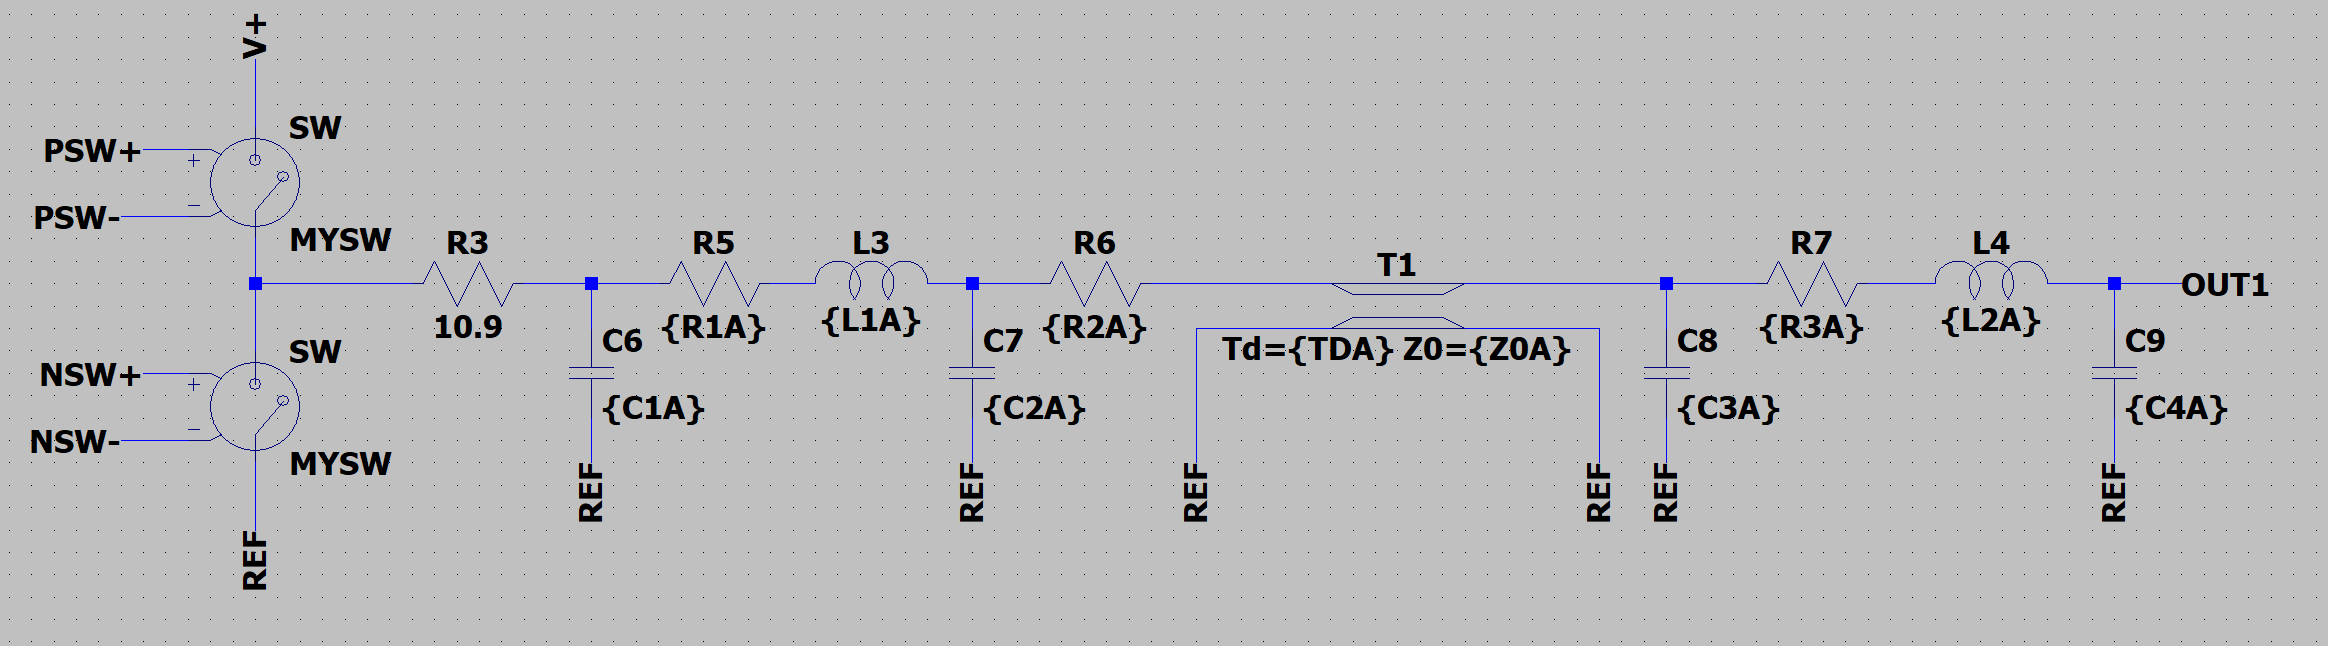
\includegraphics[width=0.9\textwidth]{ltspice_model.png}}
    \caption{LTSpice model of the driver and receiver.}
    \label{fig:driver}
\end{figure}

\newpage

\begin{table}[h]
    \centering
    \begin{tabular}{l|l r}
        \toprule[1pt]
        \textbf{Component} & \textbf{Description} & \textbf{Source}\\
        \midrule
        $SW$    & CMOS totem pole output.       & \\
        $R_3$   & 74ALVC driver resistance      & \\
        $C_6$   & 74ALVC244 driver capacitance  & (IBIS) \\
        $R_5$   & Driver package resistance     & (IBIS) \\
        $L_3$   & Driver package inductance     & (IBIS) \\
        $C_7$   & Driver package capactiance    & (IBIS) \\
        $R_6$   & Board resistor                & (Board schematic)\\
        $T_1$   & PCB trace transmission line   & \\
        $C_8$   & Receiver package capacitance  & (IBIS) \\
        $R_7$   & Receiver package resistance   & (IBIS) \\
        $L_4$   & Receiver package inductance   & (IBIS) \\
        $C_9$   & Receiver input capactitance   & (IBIS) \\
        \bottomrule[1pt]
    \end{tabular}
    \caption{System model components descriptions.}
    \label{tab:driver}
\end{table}

\textbf{Note:} physical resistor $R_6$ is not present on all lines, in which case it will be set to 0.

\subsubsection{Probe Model}

As seen in the schematic the probe is attached to the 8th output of the buffer, which can either be set to low or high. We neglect the probes capacitances/inductances and simply model it as a $50\si{\Omega}$ resistor. The model is shown in Figure \ref{fig:probe}.

\begin{figure}[h]
    \centering
    \fbox{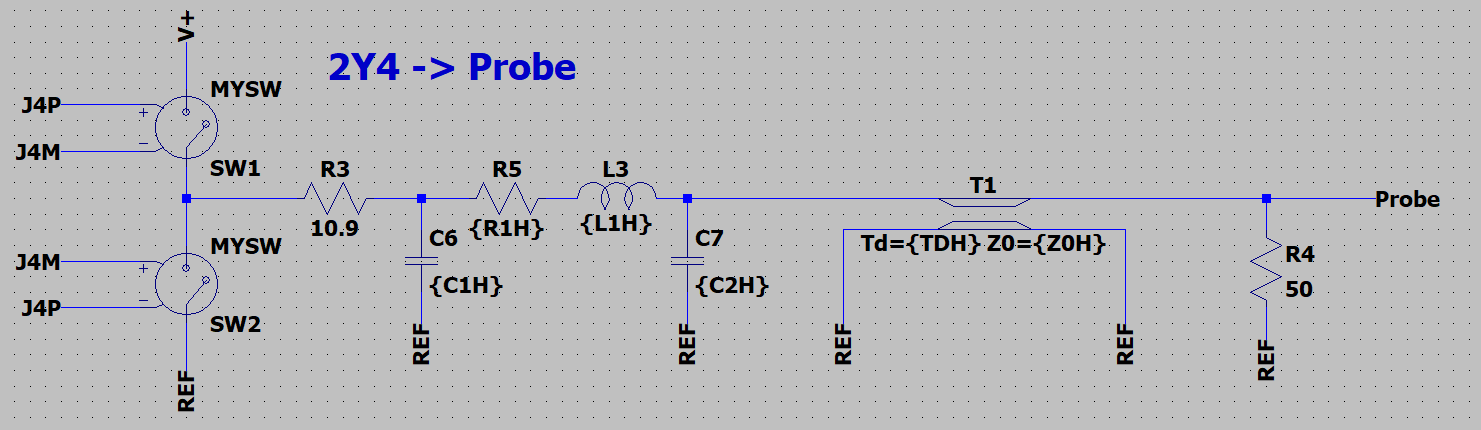
\includegraphics[width=0.9\textwidth]{probe.png}}
    \caption{LTSpice model of the probe.}
    \label{fig:probe}
\end{figure}

\subsubsection{Complete Model}

Finally we combine all the models into a single schematic. The complete model is shown in Figure \ref{fig:complete}. All 7 lines and the quiet probe line are modeleed. By configuring the voltage sources to the left we can switch 1, 3 or 7 of the lines. 

\newpage

\begin{figure}[h]
    \centering
    \fbox{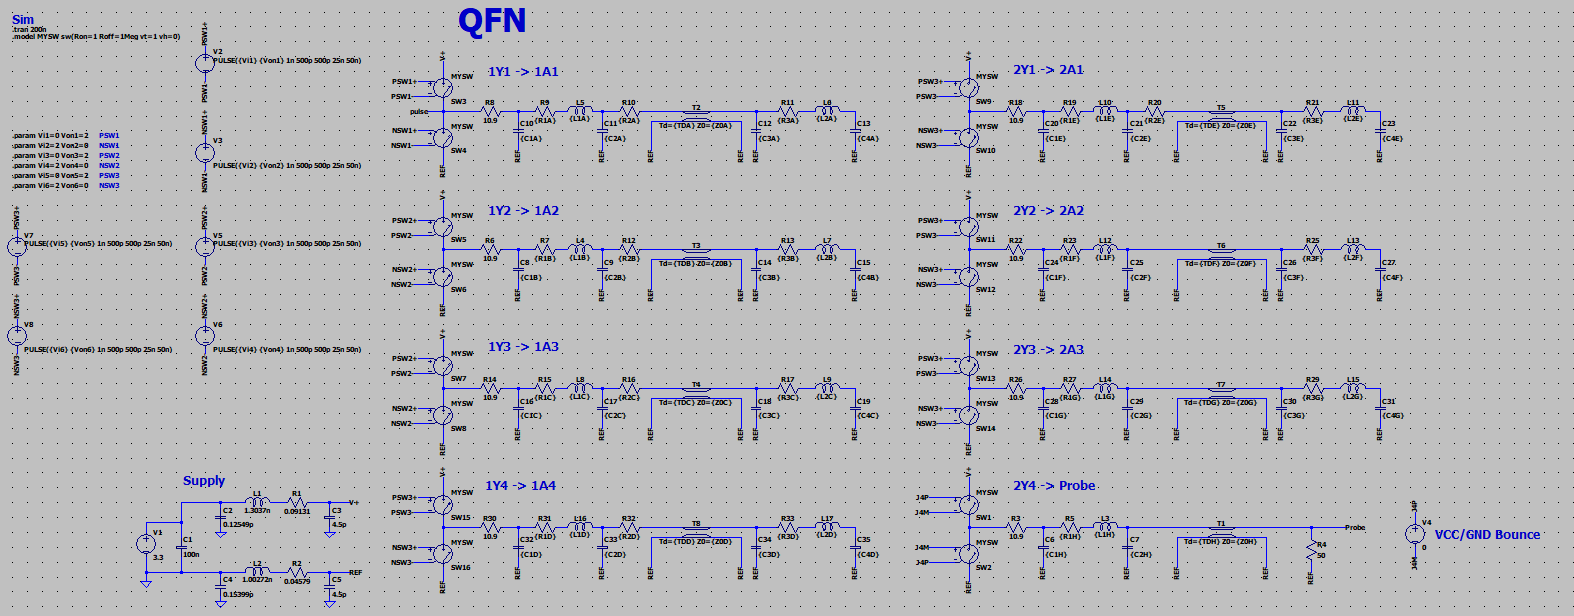
\includegraphics[width=0.9\textwidth]{complete.png}}
    \caption{LTSpice model of system.}
    \label{fig:complete}
\end{figure}

\subsection{Task 1.2}

Determine from the IBIS model for the driver/receiver IC the inductances of the signal, GND and VCC pins for the QFN and SOIC packages.

\solution

The package parameters for both the QFN and SOIC packages are shown in Table \ref{tab:pkg-params}. The values are averages of all input/output pins. In addition the output capacitance of the driver is $C_{driver} = 6.03 \si{pF}$ and input capacitance of the receiver is $C_{receiver} = 4.21 \si{pF}$. The output resistance of the driver is $10.9\si{\Omega}$.

\begin{table}[h]
    \centering
    \begin{tabular}{r|r r r r}
        \toprule[1pt]
        \textbf{Package} & \textbf{Pin} & $R_{pkg}$ [$\si{\Omega}$] & $C_{pkg}$ [$\si{pF}$] & $L_{pkg}$ [$\si{nH}$] \\
        \midrule
        SOIC  & 1Y1  & 0.034 & 0.731 & 4.714 \\
        SOIC  & 1Y2  & 0.036 & 0.533 & 4.130 \\
        SOIC  & 1Y3  & 0.035 & 0.596 & 4.414 \\
        SOIC  & 1Y4  & 0.045 & 0.868 & 5.561 \\
        SOIC  & 2Y1  & 0.040 & 0.865 & 5.518 \\
        SOIC  & 2Y2  & 0.034 & 0.583 & 4.284 \\
        SOIC  & 2Y3  & 0.036 & 0.533 & 4.130 \\
        SOIC  & 2Y4  & 0.034 & 0.732 & 4.714 \\
        \midrule
        SOIC  & 1A1  & 0.043 & 0.867 & 5.542 \\
        SOIC  & 1A2  & 0.034 & 0.591 & 4.377 \\
        SOIC  & 1A3  & 0.035 & 0.530 & 4.111 \\
        SOIC  & 1A4  & 0.034 & 0.726 & 4.634 \\
        SOIC  & 2A1  & 0.041 & 0.861 & 6.281 \\
        SOIC  & 2A2  & 0.033 & 0.742 & 4.778 \\
        SOIC  & 2A3  & 0.035 & 0.533 & 4.110 \\
        SOIC  & VCC  & 0.042 & 0.864 & 6.308 \\
        SOIC  & GND  & 0.043 & 0.866 & 6.349 \\
        \bottomrule[1pt]
    \end{tabular}
    \caption{Pin-wise package parameters for the 74ALVC244 buffer (SOIC).}
\end{table}

\begin{table}[h]
    \centering
    \begin{tabular}{r|l r r r}
        \toprule[1pt]
        \textbf{Package} & \textbf{Pin} & $R_{pkg}$ [$\si{\Omega}$] & $C_{pkg}$ [$\si{pF}$] & $L_{pkg}$ [$\si{nH}$] \\
        \midrule
        QFN  & 1Y1  & 0.0973 & 0.138 & 1.40 \\
        QFN  & 1Y2  & 0.0933 & 0.128 & 1.33 \\
        QFN  & 1Y3  & 0.100  & 0.140 & 1.44 \\
        QFN  & 1Y4  & 0.118  & 0.159 & 1.73 \\
        QFN  & 2Y1  & 0.110  & 0.151 & 1.62 \\
        QFN  & 2Y2  & 0.0960 & 0.137 & 1.38 \\
        QFN  & 2Y3  & 0.0932 & 0.127 & 1.34 \\
        QFN  & 2Y4  & 0.102  & 0.144 & 1.48 \\
        \midrule
        QFN  & 1A1  & 0 & 0 & 0 \\
        QFN  & 1A2  & 0 & 0 & 0 \\
        QFN  & 1A3  & 0 & 0 & 0 \\
        QFN  & 1A4  & 0 & 0 & 0 \\
        QFN  & 2A1  & 0 & 0 & 0 \\
        QFN  & 2A2  & 0 & 0 & 0 \\
        QFN  & 2A3  & 0 & 0 & 0 \\
        QFN  & VCC  & 0 & 0 & 0 \\
        QFN  & GND  & 0 & 0 & 0 \\
        \bottomrule[1pt]
    \end{tabular}
    \caption{Pin-wise package parameters for the 74ALVC244 buffer (SOIC).}
\end{table}

\newpage

\subsection{Task 1.3}
Simulate and document the voltages at the driver and receiving end on one of the switching outputs, as well as the quiet line. 
\subsubsection{QFN Package}

\begin{figure}[h]
    \centering
    \fbox{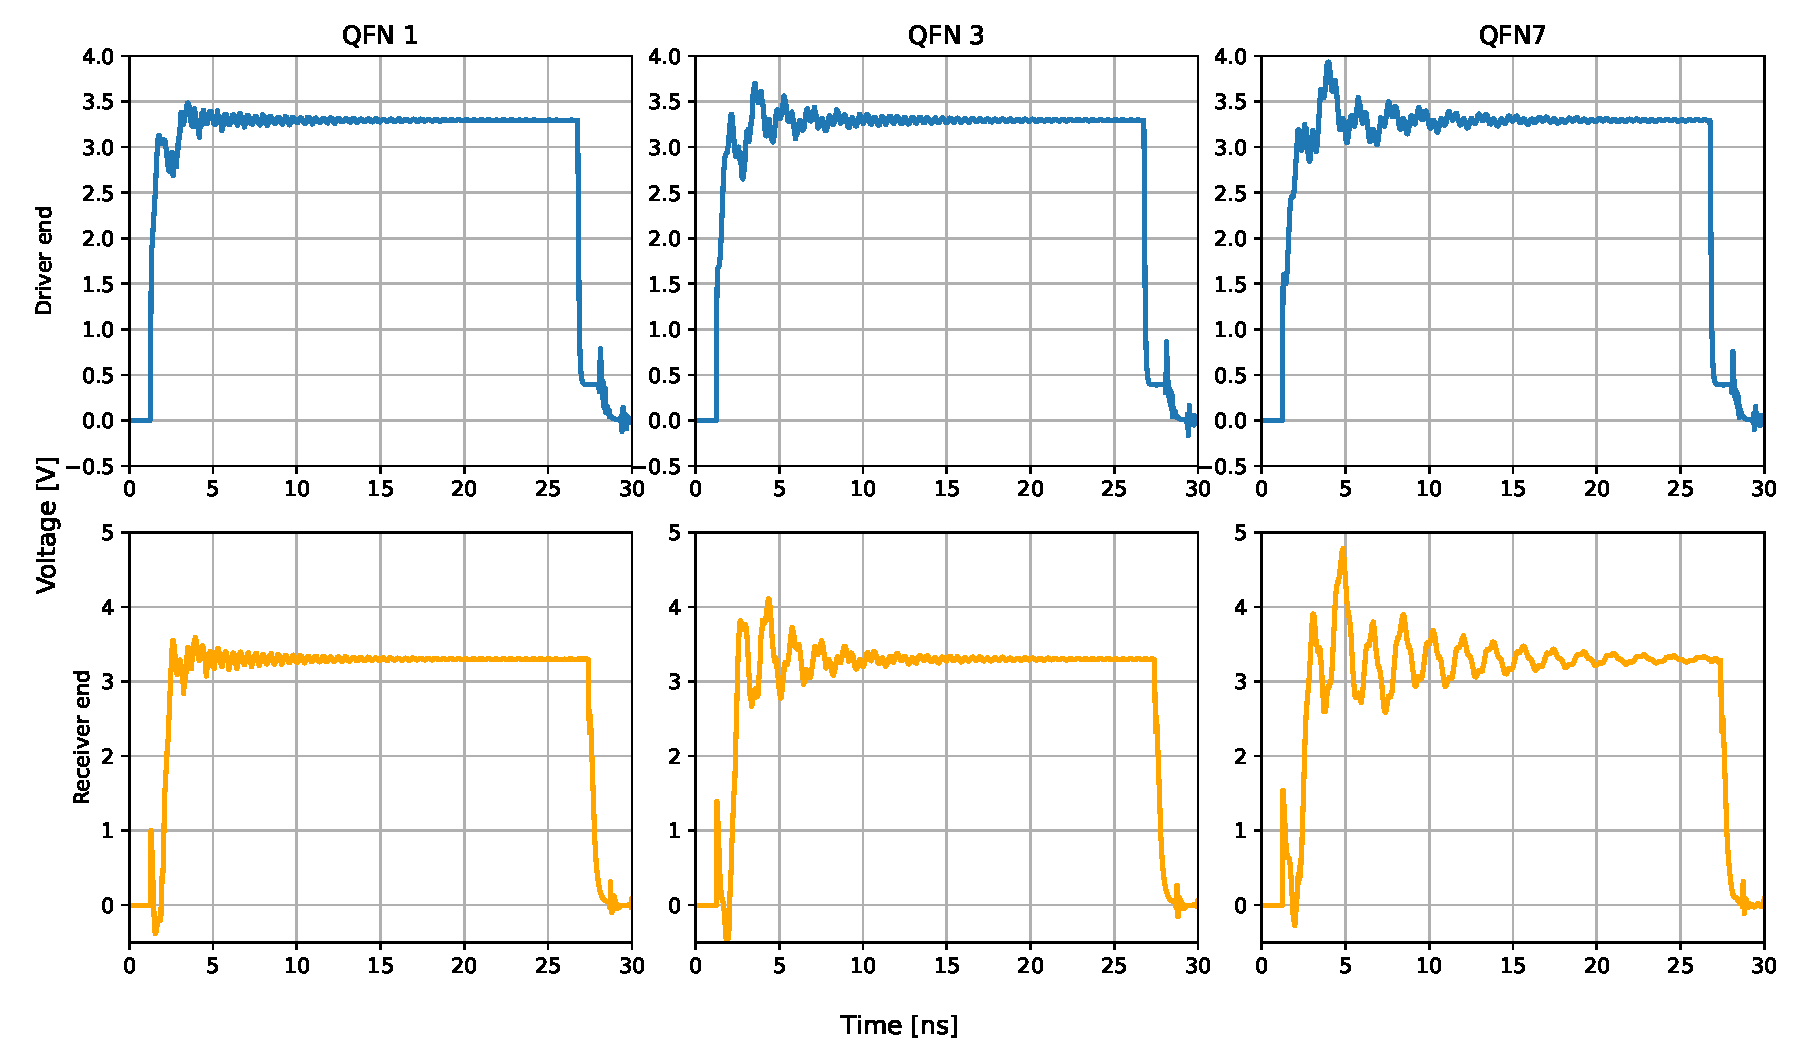
\includegraphics[width=0.9\textwidth]{qfn_sim_near_far.pdf}}
    \caption{LTSpice simulation of a switching line on the QFN package.}
    \label{fig:qfn_sim_near_far}
\end{figure}
\begin{figure}[h]
    \centering
    \fbox{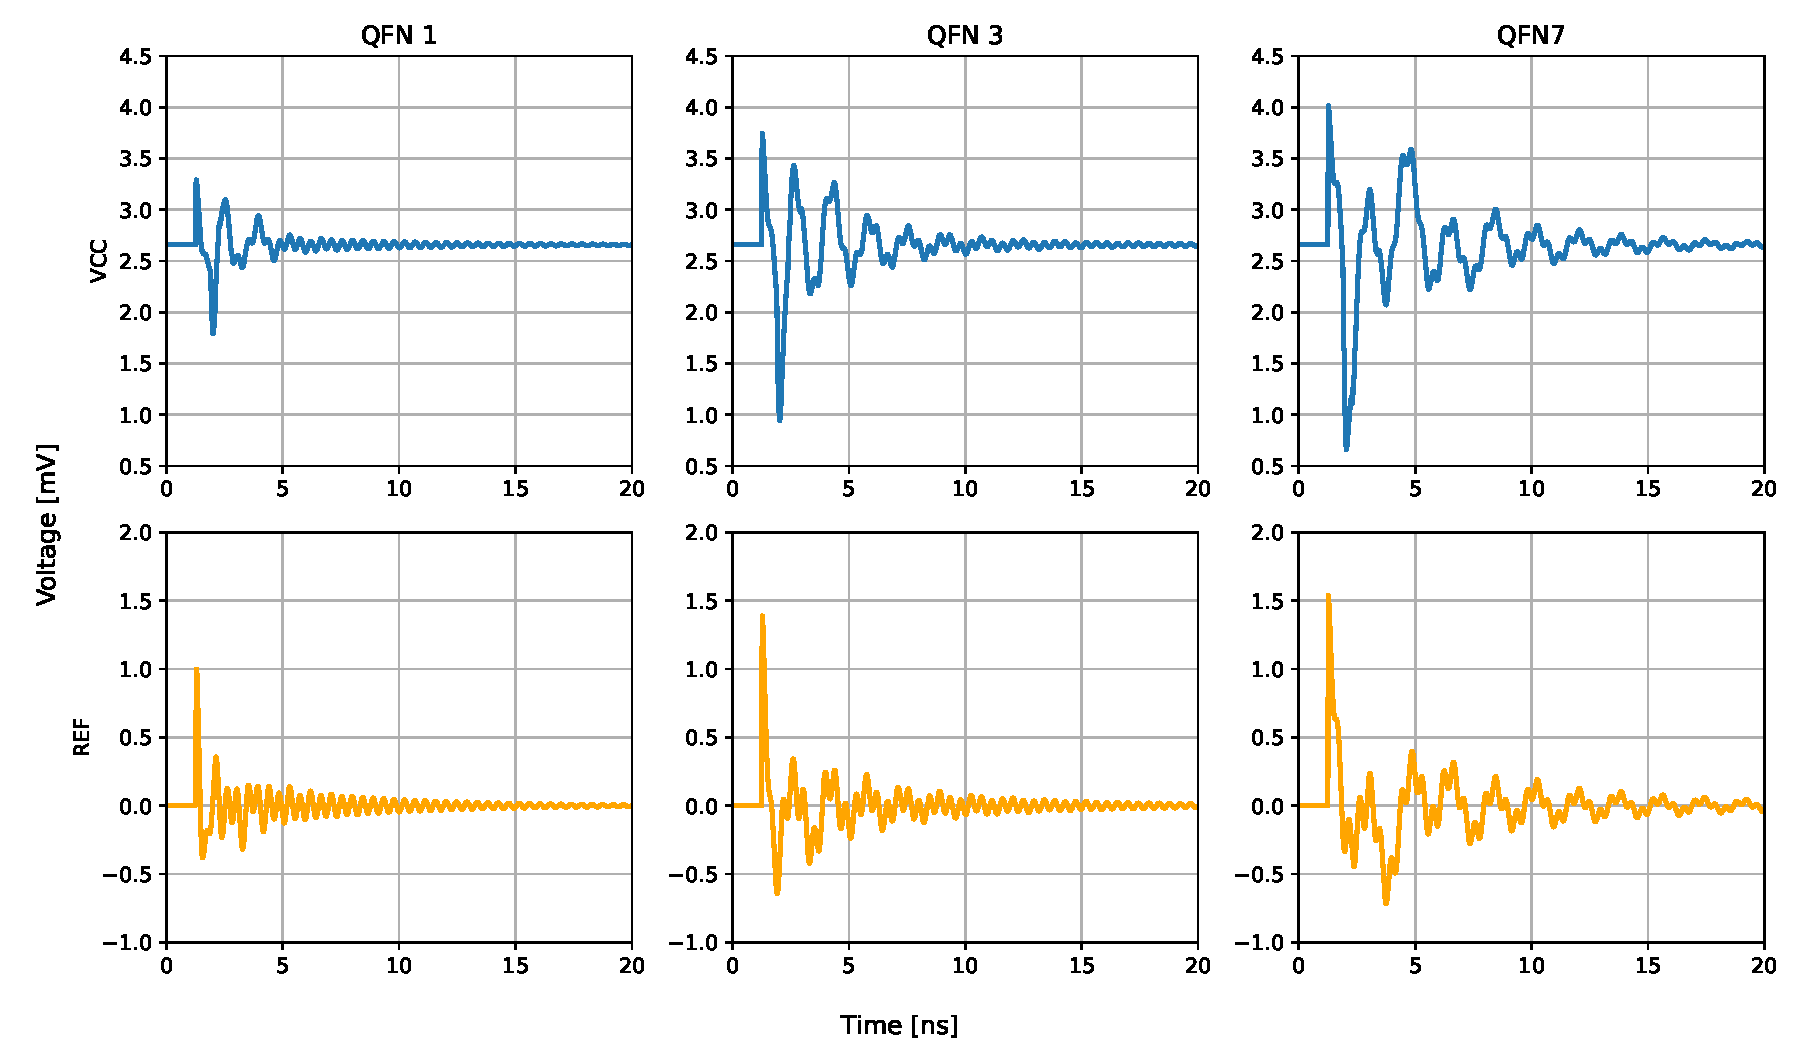
\includegraphics[width=0.9\textwidth]{qfn_sim_quiet.pdf}}
    \caption{LTSpice simulation of the quiet line on the QFN package.}
    \label{fig:qfn_sim_quiet}
\end{figure}

\begin{table}[h]
    \centering
    \begin{tabular}{r|c c}
        \toprule[1pt]
        \textbf{Outputs} & \textbf{Switching Line[V]} &\textbf{Quiet Line[V]} \\
        \midrule
        1  & 3.59  & 3.32 \\
        3  & 4.13  & 3.69 \\
        7  & 4.78  & 4.05  \\
        \bottomrule[1pt]
    \end{tabular}
    \caption{Critical voltages for the QFN package}
\end{table}

\newpage

\subsubsection{SOIC Package}

\begin{figure}[h]
    \centering
    \fbox{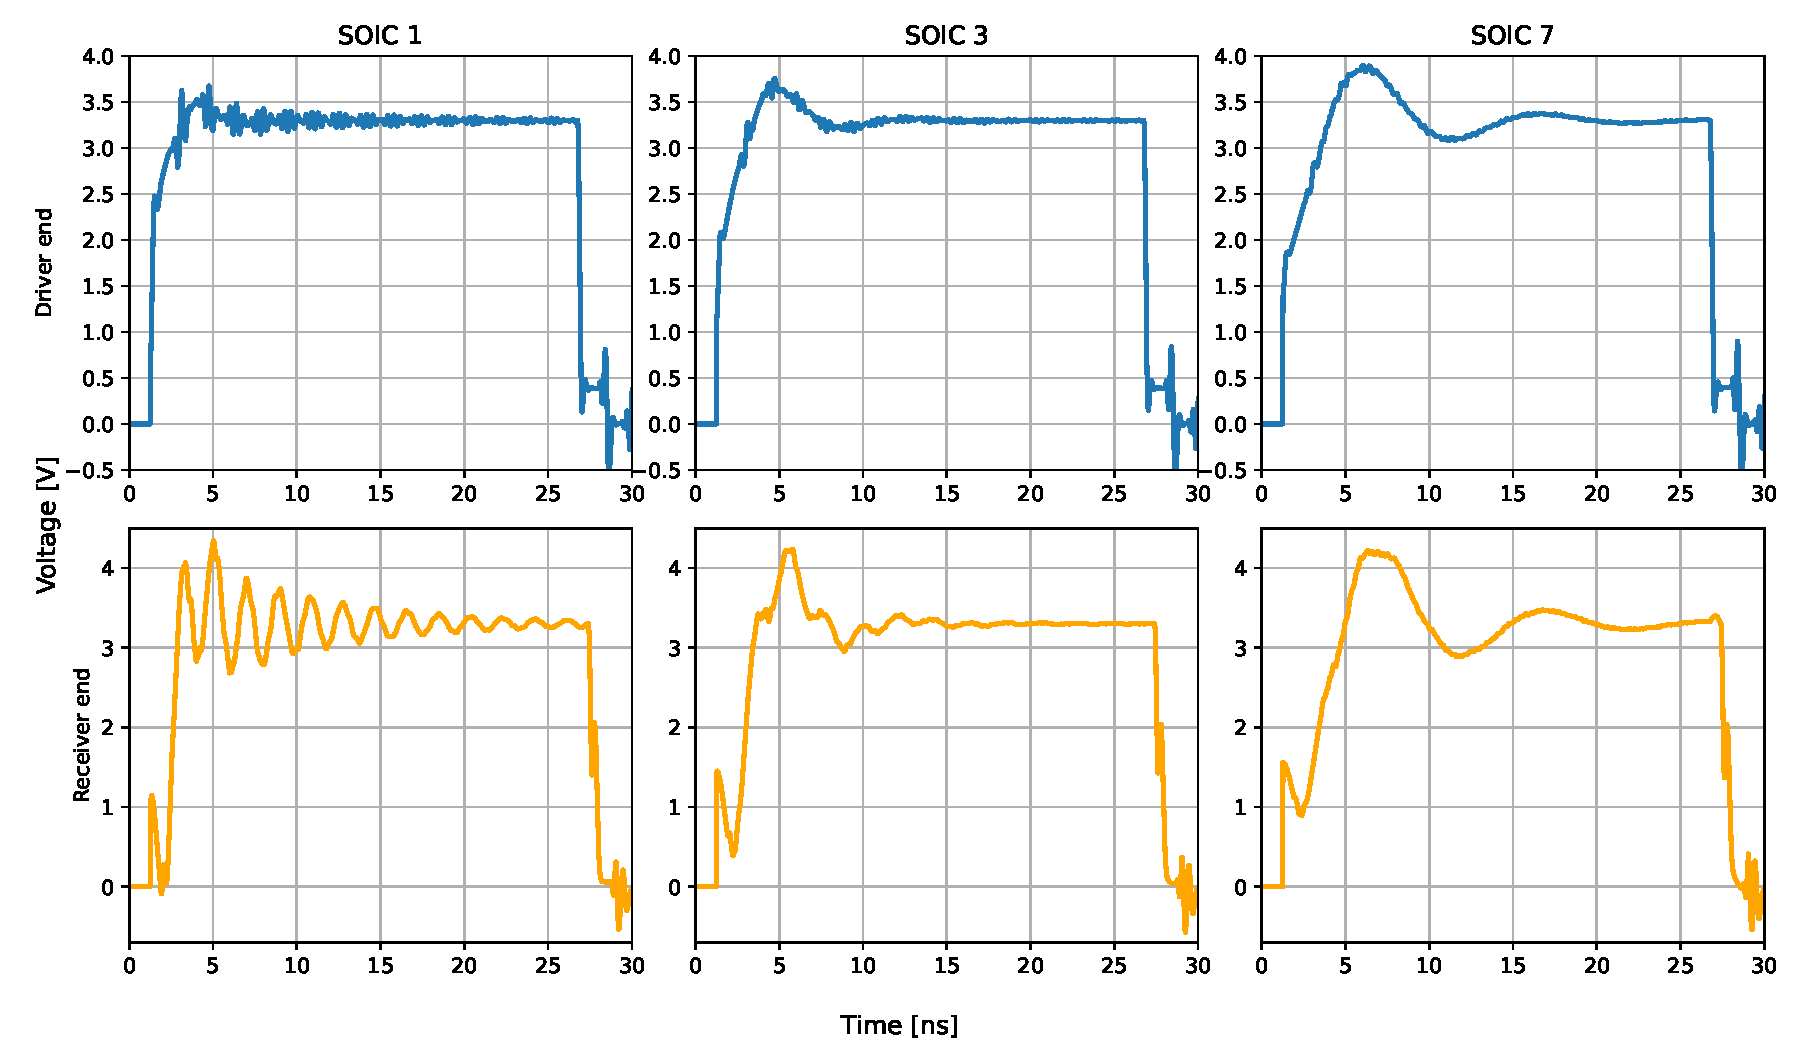
\includegraphics[width=0.9\textwidth]{soic_sim_near_far.pdf}}
    \caption{LTSpice simulation of a switching line on the SOIC package.}
    \label{fig:soic_sim_near_far}
\end{figure}
\begin{figure}[h]
    \centering
    \fbox{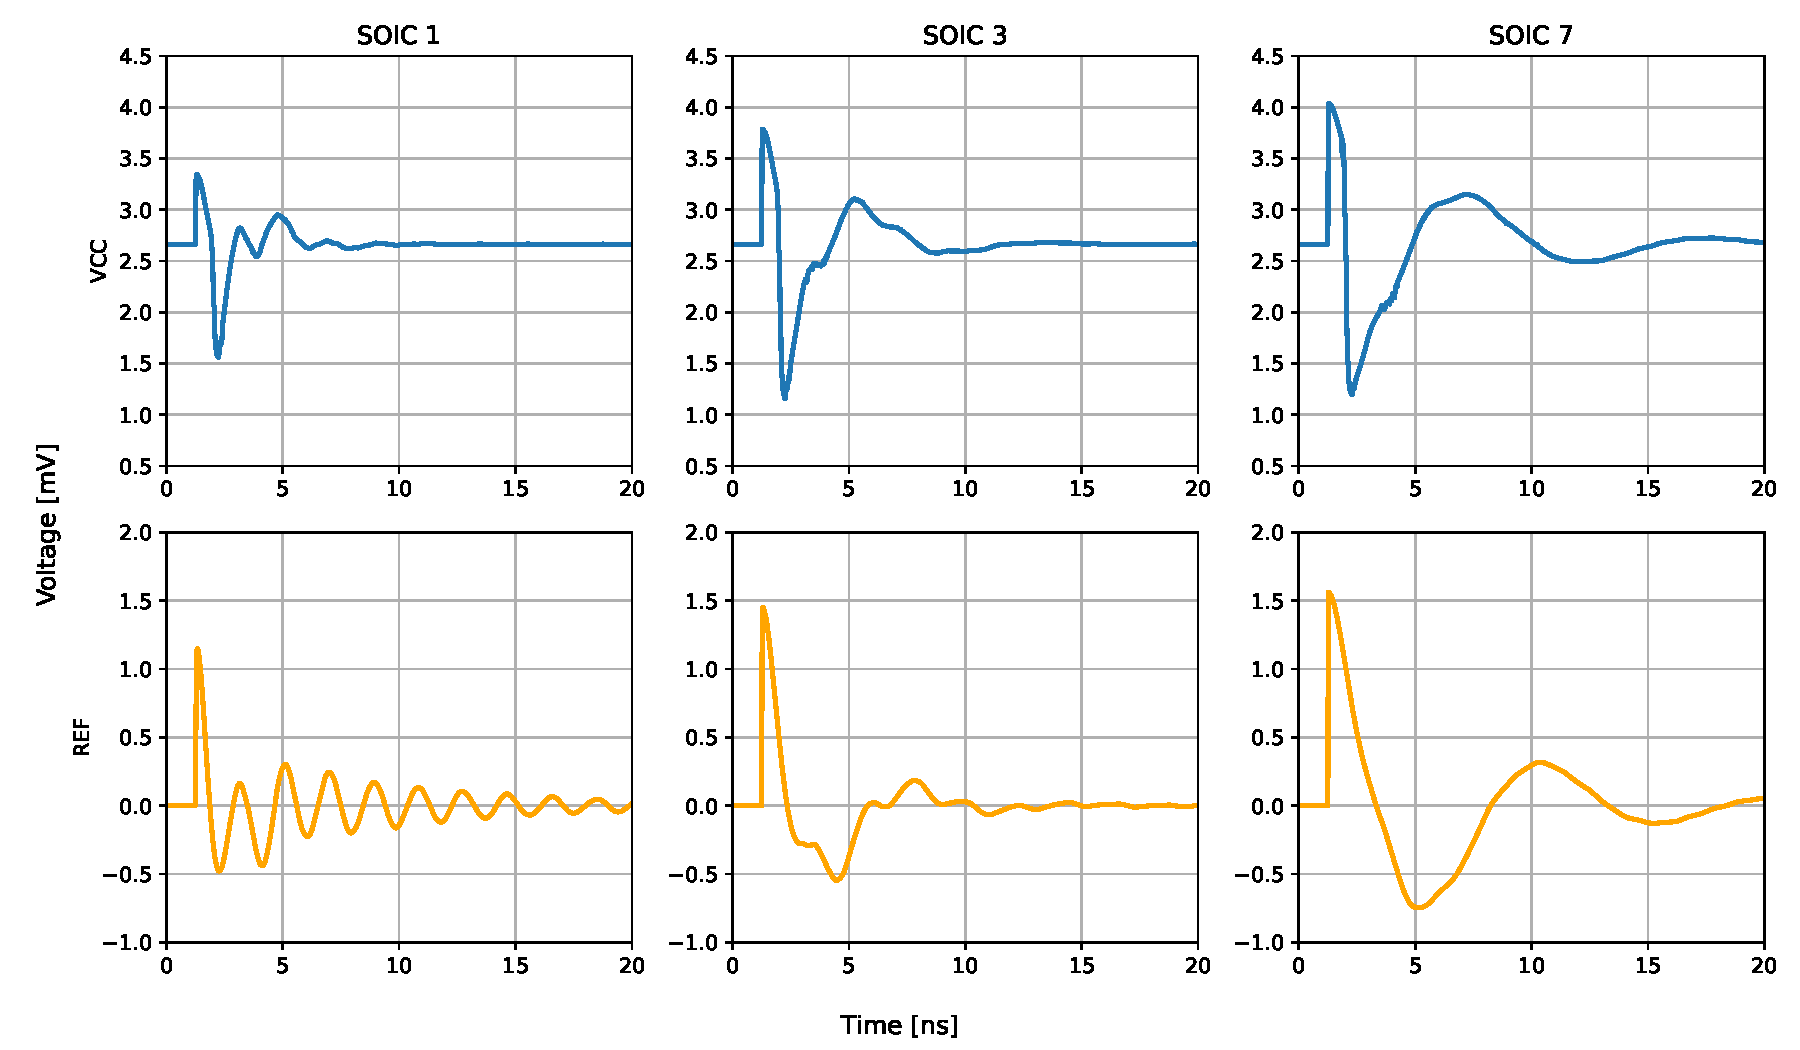
\includegraphics[width=0.9\textwidth]{soic_sim_quiet.pdf}}
    \caption{LTSpice simulation of the quiet line on the SOIC package.}
    \label{fig:soic_sim_quiet}
\end{figure}

\begin{table}[h]
    \centering
    \begin{tabular}{r|c c}
        \toprule[1pt]
        \textbf{Outputs} & \textbf{Switching Line[V]} &\textbf{Quiet Line[V]} \\
        \midrule
        1  & 4.34  & 3.37 \\
        3  & 4.24  & 3.68 \\
        7  & 4.22  & 4.01  \\
        \bottomrule[1pt]
    \end{tabular}
    \caption{Critical voltages for the SOIC package}
\end{table}

\end{document}
